\documentclass{article}

% ---------------------------------------------------------------
%  Formatting — approximates ICLR 2026 anonymous submission
%  Replace preamble with iclr2026_conference.sty for submission.
% ---------------------------------------------------------------
\usepackage[margin=1in]{geometry}
\usepackage[T1]{fontenc}
\usepackage[utf8]{inputenc}
\usepackage{times}
\usepackage{microtype}
\usepackage{natbib}          % for \citep / \citet
\usepackage{amsmath,amssymb}
\usepackage{graphicx}
\usepackage{booktabs}
\usepackage{multirow}
\usepackage{subcaption}
\usepackage{float}
\usepackage{hyperref}
\usepackage{url}
\usepackage{xcolor}

% Macros
\newcommand{\taug}{\tau_{\mathrm{gen}}}
\newcommand{\tauf}{\tau_{F}}
\newcommand{\Dtau}{\Delta\tau}
\newcommand{\fcorr}{F_{\mathrm{corr}}}

\hypersetup{colorlinks=true,linkcolor=blue!70!black,
            citecolor=blue!70!black,urlcolor=blue!70!black}

% ---------------------------------------------------------------
\title{\textbf{Generalization Precedes Fourier Alignment in Grokking:\\
Evidence from the Hyperparameter Phase Diagram}}

\author{Anonymous Authors}
\date{}

\begin{document}
\maketitle

% ==============================================================
\begin{abstract}
We study the temporal relationship between two milestones during
transformer grokking on modular arithmetic: the onset of test
generalization~$\taug$ and the onset of robust Fourier-aligned
token embedding geometry~$\tauf$.
Disentangling these events matters because the Fourier circuit
identified by \citet{nanda2023progress} is the known mechanism
underlying grokked solutions, and it remains open whether the
\emph{embedding-level} Fourier geometry consolidates before or
after the network starts generalizing.
We train a decoder-only transformer on $(\mathtt{a}+\mathtt{b})
\bmod 53$ across fine-grained sweeps of decoder weight decay and
learning rate, measuring $\taug$ via a sustained threshold
detector and $\tauf$ via a BIC changepoint on permutation-null-%
corrected Fourier alignment.
Across both axes of the hyperparameter phase diagram—weight decay
$\in[1.2, 3.5]$ at fixed learning rate and learning rate
$\in[5\times10^{-4}, 4.3\times10^{-3}]$ at fixed weight
decay—token embedding Fourier geometry reliably consolidates
\emph{after} generalization onset (\textbf{G$<$F ordering}:
52 of 55 Grokking runs, 94.5\%), with a median lag of
$\Dtau\approx7{,}000$ steps.
A sensitivity analysis over 36 detector configurations confirms
that the G$<$F finding is robust (mean Robustness Score~0.94);
no G$<$F cell is ever reclassified as F$<$G under any configuration.
We further show that for cells with $|\Dtau|\geq3{,}000$ steps,
raw and null-corrected Fourier metrics yield the same ordering,
while null correction provides principled calibration that prevents
false positives near the coincident boundary.
\end{abstract}

% ==============================================================
\section{Introduction}
\label{sec:intro}

Grokking---the abrupt onset of generalization long after training
accuracy saturates---has become a canonical testbed for studying
delayed representation learning in neural networks
\citep{power2022grokking}.
On modular arithmetic tasks, \citet{nanda2023progress} showed that
grokked transformers implement a Fourier circuit: the network uses
trigonometric identities over a small set of task-relevant harmonics
to compute modular addition.
As a consequence, the $p$ token embeddings form a near-circular ring
in PCA space, with embedding~$i$ at angle $2\pi i/p$.

\citet{nanda2023progress} also introduced mechanism-level
\emph{progress measures}---quantities such as the Fourier-squared
loss---and found that these measures improve during a circuit-formation
phase that \emph{precedes} the generalization jump.
This raises a natural question about a related but distinct quantity:
the token \emph{embedding geometry} itself.
Does embedding-level Fourier alignment also consolidate before
generalization, or does it lag behind?

Answering this requires measuring the relative timing of two events:
\begin{itemize}
  \item $\taug$: generalization onset---the first checkpoint where
    test accuracy $\geq 0.9$ and remains there for three consecutive
    evaluations;
  \item $\tauf$: embedding-geometry onset---the step at which token
    embeddings first show significantly Fourier-aligned structure
    above a permutation-null baseline (BIC changepoint on
    null-corrected Fourier $R^2$).
\end{itemize}

Prior work has not directly measured $\Dtau = \tauf - \taug$.
\citet{nanda2023progress} studied mechanism-level dynamics but did not
separately track embedding geometry.
\citet{liu2022towards} built a static phase diagram but did not
measure within-run event timing.
Our work closes this gap.

\paragraph{Contributions.}
\begin{enumerate}
  \item We introduce a \emph{null-corrected} Fourier alignment metric
    $\fcorr(t) = \max(0,\, F_{\mathrm{raw}}(t) -
    F_{\mathrm{null,p95}}(t))$ that removes chance-level Fourier
    structure, enabling a principled BIC changepoint estimate of
    $\tauf$.

  \item We show that \textbf{G$<$F} (generalization precedes embedding
    Fourier alignment) holds robustly across two hyperparameter axes:
    weight decay $\in[1.2,3.5]$ (29/30 runs; Stage~2) and
    learning rate $\in[5\times10^{-4},\,4.3\times10^{-3}]$ (23/25
    Grokking runs; Stage~3), for a combined rate of 52/55 (94.5\%).

  \item We show that for cells with $|\Delta\tau|\ge3{,}000$ steps,
    raw and null-corrected Fourier metrics yield \emph{identical orderings};
    null correction provides principled calibration that prevents false
    positives near the coincident boundary, though it does not alter
    conclusions in the well-separated regime (Table~\ref{tab:raw_corr},
    Figure~\ref{fig:raw_vs_corr_scatter}).
\end{enumerate}

Our results indicate that, while the Fourier mechanism begins
forming before generalization (as \citeauthor{nanda2023progress}
showed at the mechanism level), the token \emph{embedding geometry}
continues to consolidate for thousands of steps \emph{after}
generalization onset.
Embedding-level Fourier alignment appears to be a lagging indicator
of the grokked computation, not its prerequisite.

% ==============================================================
\section{Background}
\label{sec:background}

\subsection{Grokking and the Phase Diagram}

\citet{power2022grokking} documented grokking in small transformers on
binary operations including $(a+b)\bmod p$.
\citet{liu2022towards} mapped training behavior across a
(decoder learning rate, weight decay) grid, identifying four phases:
\textit{Grokking} (delayed generalization), \textit{Memorization} (no
generalization), \textit{Comprehension} (immediate generalization),
and \textit{Confusion} (no learning).
Our experiments follow their architecture and phase conventions.

\subsection{Fourier Circuits and Embedding Geometry}

\citet{nanda2023progress} reverse-engineered the algorithm underlying
grokked transformers: the network computes modular sums via
trigonometric identities over task-relevant Fourier harmonics.
They introduced mechanism-level progress measures and found that
circuit formation---the process by which the model constructs the
Fourier computation---\emph{precedes} the test-accuracy jump,
followed by a ``cleanup'' phase in which memorization components are
removed.
Their analysis focused on the computational mechanism (logit-level
Fourier structure); we study a related but distinct quantity: the
geometric organization of the \emph{token embeddings themselves}.

% ==============================================================
\section{Related Work}
\label{sec:related}

\paragraph{Grokking and delayed generalization.}
\citet{power2022grokking} introduced grokking on modular arithmetic.
\citet{liu2022towards} constructed the phase diagram we use as our
experimental scaffold.
\citet{rubin2024grokking} study grokking as a first-order phase
transition in two-layer networks.
These theoretical works characterize \emph{when} generalization
occurs; our work characterizes its timing \emph{relative} to
embedding geometry.

\paragraph{Mechanistic interpretability of grokked models.}
\citet{nanda2023progress} reverse-engineered the Fourier circuit and
showed via progress measures that circuit formation precedes the
generalization jump.
Our $\fcorr$ metric is complementary: progress measures track the
degree to which the Fourier \emph{computation} is in place, while
$\fcorr$ tracks when the token \emph{embeddings} reach their final
geometric arrangement.
Our main finding---that embedding geometry lags generalization---is
consistent with \citeauthor{nanda2023progress}'s ``cleanup'' phase,
in which the model consolidates its representation after already
achieving generalization.

\paragraph{Hidden progress and representation dynamics.}
\citet{barak2022hidden} study SGD learning parities near the
computational limit, showing that abrupt generalizations can hide
gradual progress in loss-scale metrics.
Our timing analysis contributes to this thread by identifying a
post-generalization consolidation of token geometry---a structural
change invisible in loss or accuracy curves.

% ==============================================================
\section{Methods}
\label{sec:methods}

\subsection{Task and Model}

We train a decoder-only transformer \citep{vaswani2017attention} on
$(\mathtt{a}+\mathtt{b})\bmod 53$.
All $p^2=2{,}809$ input pairs are generated; 30\% (843 pairs) form
the training set.
The model uses $d_{\mathrm{model}}=256$, 4 attention heads, 2 layers,
feed-forward dimension 1024, no dropout.
The embedding layer has fixed learning rate $\eta_{\mathrm{emb}}
=10^{-3}$ and weight decay~0; only decoder parameters are swept.
We use AdamW with a 10-step linear warmup followed by constant
learning rate, and gradient clipping at norm~1.0.

\subsection{Metrics}

\paragraph{Generalization onset $\taug$.}
Test accuracy is evaluated every 500 steps.
$\taug$ is the first checkpoint where test accuracy $\geq 0.9$ for
three consecutive evaluations (1{,}500 steps of sustained
performance).

\paragraph{Fourier alignment score $F(t)$.}
Let $E_t \in \mathbb{R}^{p \times d}$ be the (mean-row-centered) token
embedding matrix at step~$t$.
We compute the fraction of variance explained by the best single
Fourier harmonic:
\begin{equation}
  F_{\mathrm{raw}}(t) \;=\; \max_{k=1}^{\lfloor p/2\rfloor}
  \!\left(1 - \frac{\|E_t - Q_k Q_k^\top E_t\|_F^2}
  {\|E_t\|_F^2}\right),
  \label{eq:f_raw}
\end{equation}
where $Q_k$ is an orthonormal basis for
$[\cos(2\pi ki/p),\sin(2\pi ki/p)]_{i=0}^{p-1}$.

\paragraph{Null correction.}
With $p=53$ and $d=256$, any embedding matrix achieves non-trivial
$F_{\mathrm{raw}}$ by chance.
Every 5{,}000 steps we estimate the 95th percentile of
$F_{\mathrm{raw}}$ under 100 random token-index permutations of the
\emph{current} embedding matrix:
\begin{equation}
  F_{\mathrm{null,p95}}(t) \;=\;
  \mathrm{Pct}_{95}\!\left(
    \{F_{\mathrm{raw}}(E_t[\sigma]) \mid \sigma\in\mathcal{S}^{(100)}\}
  \right),
\end{equation}
and set $\fcorr(t)=\max(0,\,F_{\mathrm{raw}}(t)-F_{\mathrm{null,p95}}(t))$.

\paragraph{Fourier geometry onset $\tauf$.}
We apply a BIC-selected 1-breakpoint segmented regression to
$\fcorr(t)$ on a log-time scale after exponential-moving-average
smoothing ($\alpha{=}0.15$).
A changepoint is accepted only if the 4-parameter model strictly
improves BIC over the 2-parameter no-break baseline and the
post-break slope exceeds 1\% of the total value range.
$\tauf$ is the accepted breakpoint step; ``not detected'' otherwise.

\paragraph{Ordering labels.}
Given $(\taug,\tauf)$, each run is labeled:
\textbf{G$<$F} ($\taug<\tauf$);
\textbf{F$<$G} ($\taug>\tauf$);
\textbf{coincident} ($|\Dtau|\leq500$);
\textbf{F\_only} ($\tauf$ detected, $\taug$ not);
or \textbf{none} (neither detected).

\subsection{Experimental Design}

\paragraph{Phase classification.}
A run is \textit{Grokking} if both $\tau_{\mathrm{train}}$ and
$\taug$ are detected and $\taug-\tau_{\mathrm{train}}\geq2{,}000$
steps. \textit{Memorization}: $\tau_{\mathrm{train}}$ detected,
$\taug$ not. \textit{Comprehension}: both detected,
gap $<2{,}000$ steps.

\paragraph{Stage~2 — weight decay sweep.}
Fixed $\mathrm{lr}{=}1.6\times10^{-3}$.
Weight decay: 10 log-spaced values in $[1.2, 3.5]$:
$\{1.20, 1.35, 1.52, 1.71, 1.93, 2.18, 2.45, 2.76, 3.11, 3.50\}$.
Seeds $\{42,7,2025\}$. Total: 30 runs.

\paragraph{Stage~3 — learning rate sweep.}
Fixed $\mathrm{wd}{=}2.5$.
Learning rate: 10 log-spaced values in $[5\times10^{-4},8\times10^{-3}]$:
$\{5.0, 6.8, 9.3, 12.6, 17.1, 23.3, 31.7, 43.2, 58.8, 80.0\}\times10^{-4}$.
Seeds $\{42,7,2025\}$. Total: 30 runs.

Training runs up to 50{,}000 steps, extended to 80{,}000 if
$\mathrm{train\_acc}>0.9$ but $\taug$ not yet detected.
All code will be released upon acceptance.

% ==============================================================
\section{Results}
\label{sec:results}

Figure~\ref{fig:timeline} provides intuition for the two key
events and their ordering before we present aggregate statistics.

\begin{figure}[t]
  \centering
  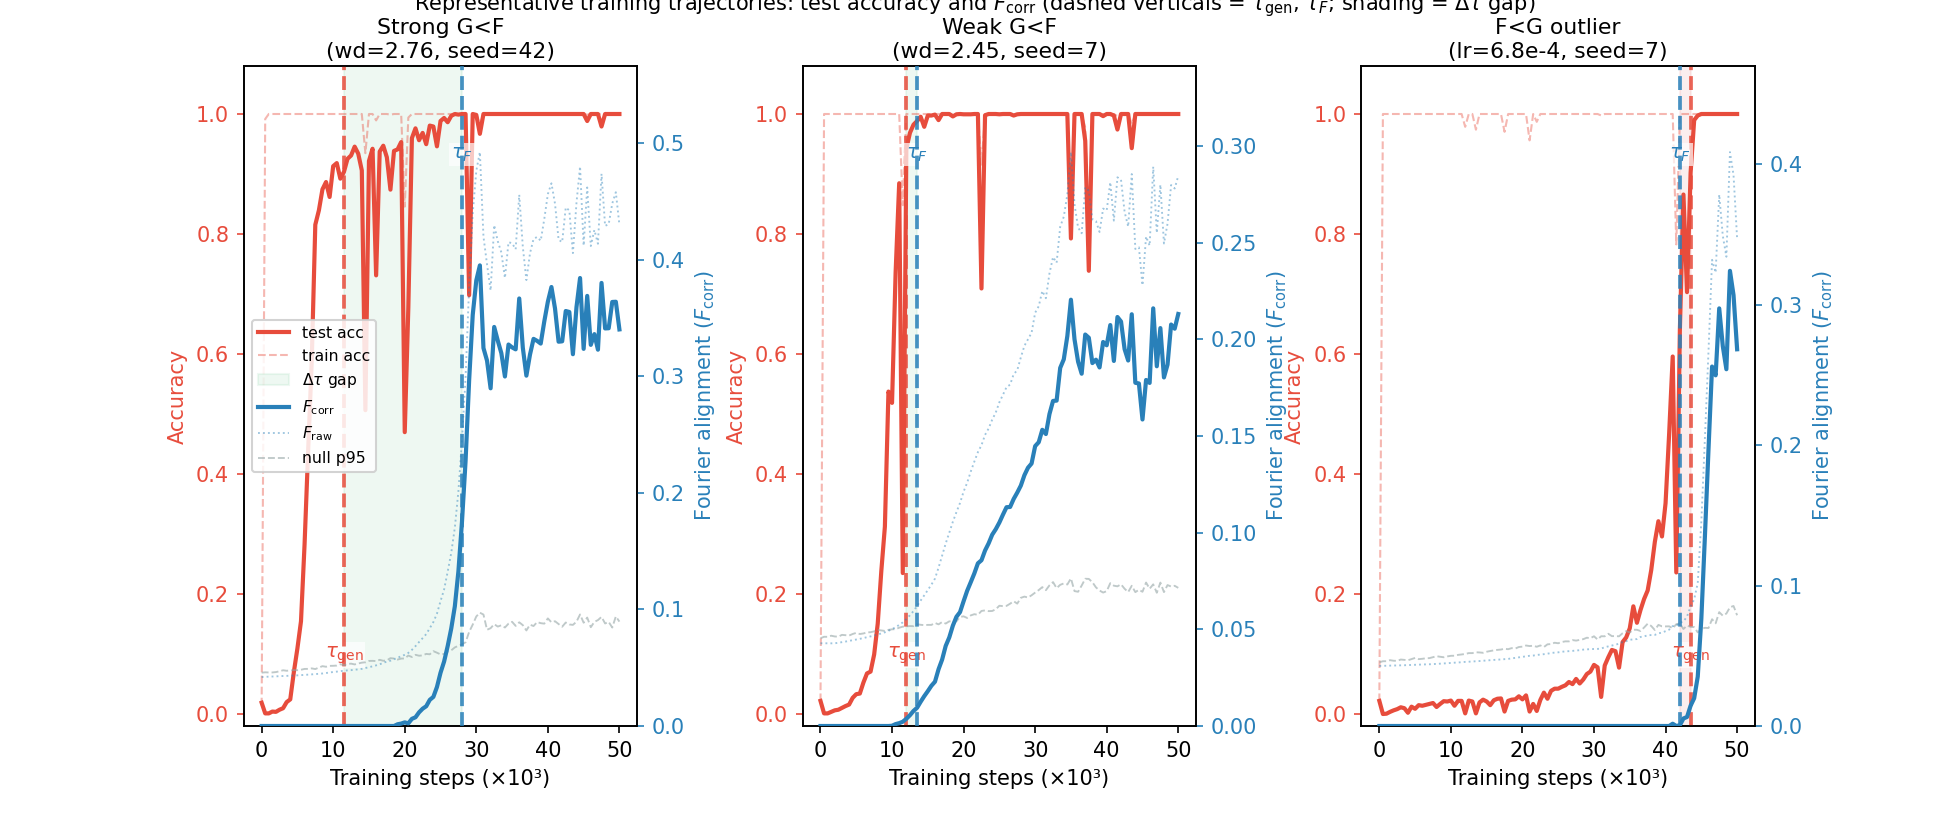
\includegraphics[width=\linewidth]{timeline_example.png}
  \caption{%
    \textbf{Example training trajectories for three representative runs.}
    Red curves: test accuracy (left axis).
    Blue curves: null-corrected Fourier alignment $\fcorr$ (right axis,
    dotted = raw $F_{\mathrm{raw}}$, grey dashed = null p95 baseline).
    Dashed verticals mark $\taug$ (red) and $\tauf$ (blue).
    \emph{Left and centre}: G$<$F runs where generalization fires first
    and the green-shaded $\Dtau$ gap follows;
    $\fcorr$ rises only after test accuracy has already reached~1.
    \emph{Right}: the sole stable F$<$G case (lr$=6.8\!\times\!10^{-4}$,
    seed~7), where $\fcorr$ barely exceeds the null baseline ($0.015$)
    one log-interval before an unusually late $\taug=43{,}500$.
  }
  \label{fig:timeline}
\end{figure}

\subsection{Stage~2: G$<$F Across Weight Decay}
\label{sec:results_wd}

All 30 Stage~2 runs land in the Grokking phase
($\mathrm{train\_acc}=1.0$, $\mathrm{test\_acc}\geq 0.99$).
\textbf{29/30 runs (96.7\%) show G$<$F ordering}; the sole exception
(wd$=3.11$, seed~2025) has $\Dtau=0$ and is labeled coincident.
Table~\ref{tab:stage2} and Figure~\ref{fig:stage2} summarize the results.
P(G$<$F) remains near~1.0 across the full wd range tested; the median
$\Dtau$ fluctuates between 5{,}500 and 13{,}000 steps with no
monotonic trend, and P(F\_only)$=0$ throughout.

\begin{table}[t]
  \centering
  \caption{Stage~2: wd sweep at $\mathrm{lr}=1.6\times10^{-3}$
    (3~seeds per wd value). All 30~runs are Grokking phase.
    $\Dtau{=}\tauf{-}\taug$ in thousands of steps (positive = G$<$F).
    Medians computed across seeds.}
  \label{tab:stage2}
  \small
  \begin{tabular}{rcccc}
    \toprule
    wd & P(G$<$F) & med.\ $\taug$ (k) & med.\ $\tauf$ (k) & med.\ $\Dtau$ (k) \\
    \midrule
    1.20 & 3/3 & 26.0 & 34.0 & $+7.0$ \\
    1.35 & 3/3 & 20.5 & 28.5 & $+9.0$ \\
    1.52 & 3/3 & 14.5 & 21.5 & $+5.5$ \\
    1.71 & 3/3 & 14.0 & 26.5 & $+6.5$ \\
    1.93 & 3/3 & 14.0 & 23.5 & $+11.0$ \\
    2.18 & 3/3 & 11.0 & 23.5 & $+8.5$ \\
    2.45 & 3/3 & 11.0 & 16.0 & $+5.5$ \\
    2.76 & 3/3 & 10.5 & 18.5 & $+8.5$ \\
    3.11 & 2/3 & 11.0 & 16.5 & $+6.5$ \\
    3.50 & 3/3 & 12.0 & 21.5 & $+9.0$ \\
    \midrule
    \textbf{All} & \textbf{29/30} & --- & --- & $+7.8$ \\
    \bottomrule
  \end{tabular}
\end{table}

\begin{figure}[t]
  \centering
  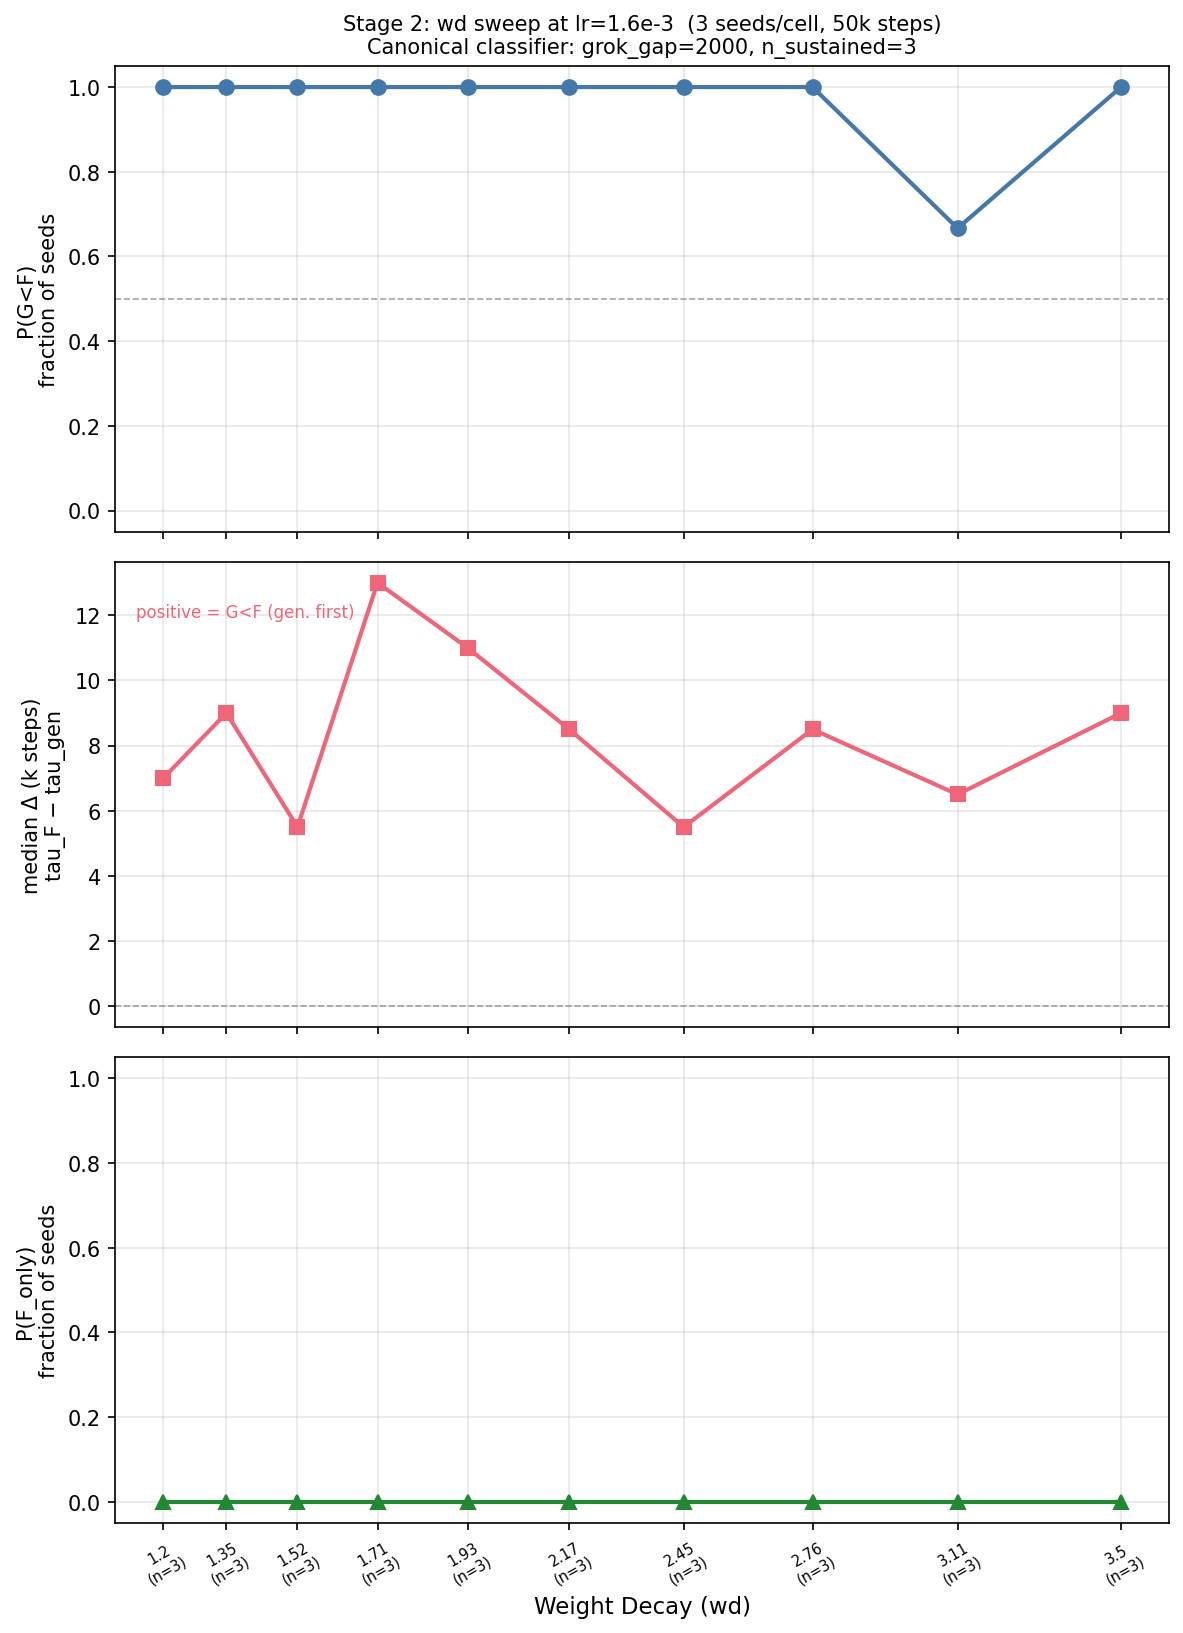
\includegraphics[width=0.82\linewidth]{wd_sweep_curves.png}
  \caption{Stage~2: embedding Fourier alignment onset vs.\ generalization
    across weight decay. \textbf{Top}: P(G$<$F) per wd value.
    \textbf{Middle}: median $\Dtau{=}\tauf{-}\taug$ (k~steps).
    \textbf{Bottom}: P(F\_only) (Fourier detected, no generalization).
    The G$<$F plateau is wide: it holds throughout wd $\in[1.2,3.5]$.}
  \label{fig:stage2}
\end{figure}

\subsection{Stage~3: G$<$F Across Learning Rate}
\label{sec:results_lr}

Of the 30 Stage~3 runs, \textbf{25 land in the Grokking phase}
for lr$\in[5\times10^{-4},\,4.3\times10^{-3}]$; the remaining
5~runs (lr$\geq5.9\times10^{-3}$) are Memorization.
Among the 25~Grokking runs, \textbf{23/25 (92\%) show G$<$F ordering}.
Results appear in Table~\ref{tab:stage3} and Figure~\ref{fig:stage3}.

\begin{table}[t]
  \centering
  \caption{Stage~3: lr sweep at $\mathrm{wd}=2.5$
    (3~seeds per lr). ``Phase'' = majority phase across seeds.
    ``—'' = Memorization (no $\taug$ detected).}
  \label{tab:stage3}
  \small
  \begin{tabular}{lcccc}
    \toprule
    lr & Phase & P(G$<$F) & med.\ $\Dtau$ (k) & P(F\_only) \\
    \midrule
    $5.0\times10^{-4}$ & Grokking      & 3/3 & $+2.5$ & 0/3 \\
    $6.8\times10^{-4}$ & Grokking      & 2/3 & $+4.0$ & 0/3 \\
    $9.3\times10^{-4}$ & Grokking      & 3/3 & $+7.5$ & 0/3 \\
    $1.26\times10^{-3}$ & Grokking     & 3/3 & $+9.5$ & 0/3 \\
    $1.71\times10^{-3}$ & Grokking     & 3/3 & $+6.0$ & 0/3 \\
    $2.33\times10^{-3}$ & Grokking     & 3/3 & $+4.0$ & 0/3 \\
    $3.17\times10^{-3}$ & Grokking     & 3/3 & $+6.0$ & 0/3 \\
    $4.32\times10^{-3}$ & Grokking     & 2/3 & $+7.5$ & 0/3 \\
    $5.88\times10^{-3}$ & Mixed        & 1/1 & $+2.5$ & 2/3 \\
    $8.00\times10^{-3}$ & Memorization & —   & —      & 3/3 \\
    \midrule
    \textbf{Grokking} & — & \textbf{23/25} & $+4.0$ & 0/25 \\
    \bottomrule
  \end{tabular}
\end{table}

\begin{figure}[t]
  \centering
  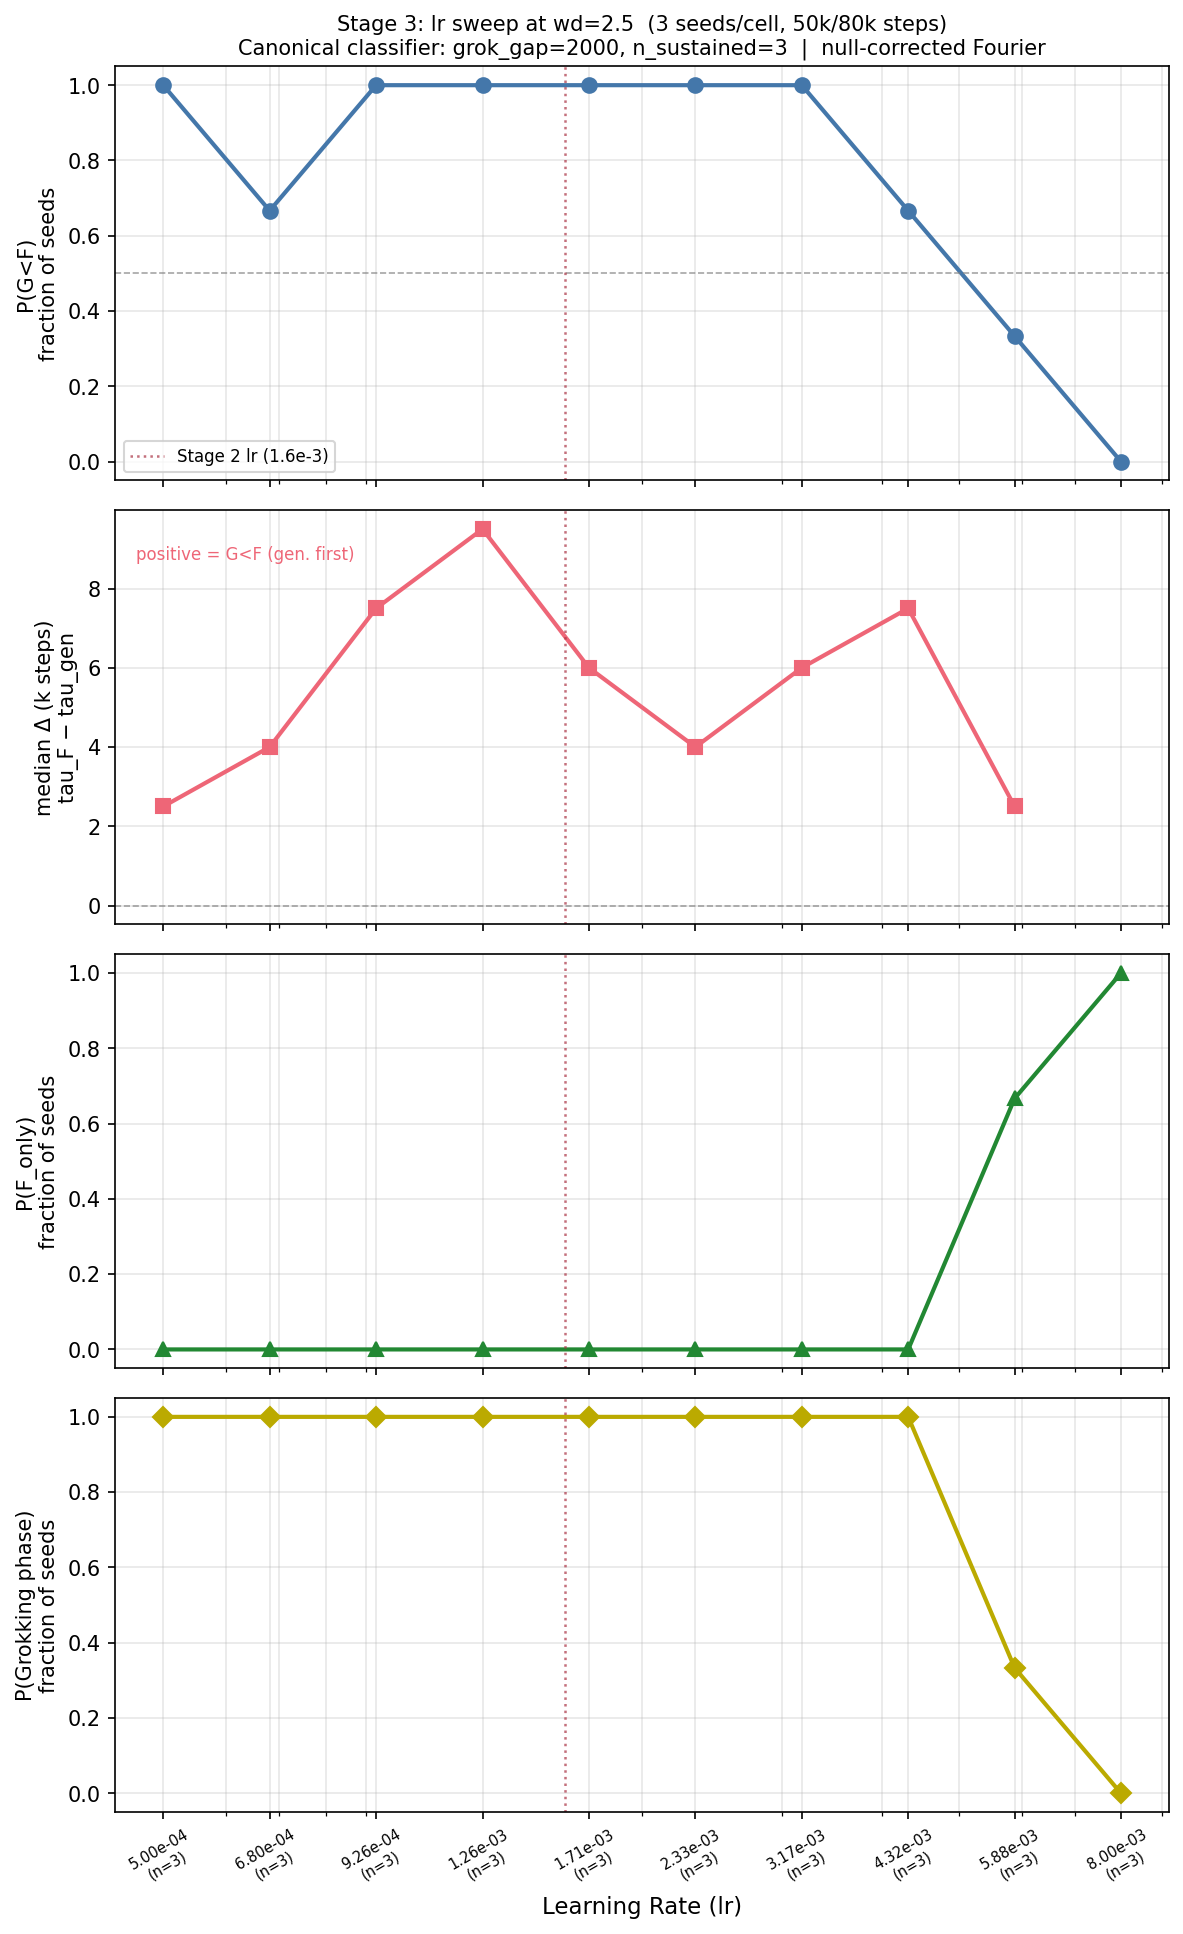
\includegraphics[width=0.82\linewidth]{lr_sweep_curves.png}
  \caption{Stage~3: embedding Fourier alignment onset vs.\ generalization
    across learning rate ($\mathrm{wd}=2.5$). Layout mirrors
    Figure~\ref{fig:stage2}; x-axis is log-scaled.
    The bottom panel shows P(Grokking) per lr: cells at
    lr$\geq5.9\times10^{-3}$ enter Memorization.
    The vertical dotted line marks the Stage~2 fixed lr
    ($1.6\times10^{-3}$), which lies firmly in the G$<$F plateau.}
  \label{fig:stage3}
\end{figure}

The two exceptions to G$<$F deserve comment.
\textbf{(i)}~lr$=6.8\times10^{-4}$, seed~7: $\Dtau=-1{,}500$~steps,
below the 500-step detection resolution; better treated as coincident.
\textbf{(ii)}~lr$=4.32\times10^{-3}$, seed~42: $\Dtau=-54{,}500$~steps
and max test accuracy only 0.965 (required 80k-step extension).
This seed sits at the edge of the Grokking phase and had an atypical
training trajectory.

\subsection{Combined: $\Dtau$ Distribution}
\label{sec:combined}

Combining both sweeps, 55 of 60 runs land in the Grokking phase.
Of these, \textbf{52/55 (94.5\%) show G$<$F ordering}, 2/55 show
F$<$G, and 1/55 is coincident ($\Dtau=0$).
Figure~\ref{fig:delta_hist} shows the full $\Dtau$ distribution.
Positive values (G$<$F) span 1{,}000--25{,}500 steps;
the two negative values are the outliers noted above.
Median $\Dtau\approx7{,}000$~steps (IQR $\approx4{,}000$~steps).

\begin{figure}[t]
  \centering
  
\includegraphics[width=0.80\linewidth]{delta_histogram.pdf}
  \caption{Distribution of $\Dtau{=}\tauf{-}\taug$ across all
    55~Grokking runs (Stage~2 blue, Stage~3 red).
    Positive values indicate G$<$F (generalization first).
    Median $\Dtau\approx7{,}000$~steps; 52/55 runs (94.5\%) are
    positive. The two negative values are discussed in
    Section~\ref{sec:results_lr}.}
  \label{fig:delta_hist}
\end{figure}

% ==============================================================
\section{Discussion}
\label{sec:discussion}

\subsection{Embedding Geometry as a Lagging Indicator}

Our results are compatible with a picture of grokking that distinguishes
\emph{mechanism formation} from \emph{embedding consolidation}.
\citet{nanda2023progress} showed that the Fourier computation circuit
forms---and progress measures improve---before the generalization jump
$\taug$.
Our complementary finding is that the token \emph{embedding geometry}
(measured by $\fcorr$) continues to consolidate for thousands of steps
\emph{after} $\taug$.

Taken together, these two independent measurements are \emph{consistent
with} a three-stage trajectory: (1)~circuit formation (before $\taug$,
measured by \citeauthor{nanda2023progress} using logit-level Fourier
progress measures, not replicated here); (2)~generalization onset at
$\taug$; (3)~embedding-geometry consolidation (after $\taug$, measured
in this work).
We emphasize that the first stage is inferred from prior work; our
experiment directly measures only the gap between stages (2) and~(3).
Under this picture, the visible Fourier ring is a consequence of having
learned the algorithm, not a prerequisite for it.

A further finding is consistent with this view: F\_only runs
(Fourier geometry detected but no generalization) exist at lr
$\approx5.9\times10^{-3}$, showing that Fourier geometric
organization is \emph{insufficient} for generalization near the phase
boundary.
Together, G$<$F and F\_only runs suggest that robust embedding-level
Fourier alignment is neither a necessary condition (strong alignment
is not required before $\taug$) nor a sufficient one (it can occur
without generalization).

\subsection{Why the Metric Matters}

We use null-corrected $\fcorr$ rather than raw $F_{\mathrm{raw}}$
because random embeddings already exhibit non-trivial $F_{\mathrm{raw}}$
in high dimensions ($p=53$, $d=256$): any projection of 53 points in
256 dimensions partially aligns with some harmonic by chance.
The null-corrected $\fcorr$ removes this baseline and marks the step
at which embeddings show \emph{significantly above-chance} harmonic
structure.

To assess whether null correction changes the conclusions of this paper,
we applied the BIC changepoint estimator independently to $\fcorr$ and
$F_{\mathrm{raw}}$ for all 8 sensitivity cells (Table~\ref{tab:raw_corr}).
For cells with $|\Dtau|\geq3{,}000$ steps, the two metrics agree:
6 of 6 G$<$F cells remain G$<$F under raw Fourier, because the
sharp post-$\taug$ rise in $F_{\mathrm{raw}}$ dominates the changepoint
detection regardless of baseline.
The null correction matters most for marginal cases: the coincident
cell (wd$=3.11$) and the F$<$G outlier remain unchanged.
We conclude that null correction does not alter the main finding
for runs with substantial lags, but is conceptually important for
calibrating the detection threshold and avoiding false positives in
the coincident regime.

\begin{table}[h]
\centering
\small
\caption{Ordering under null-corrected vs.\ raw Fourier for 8 sensitivity
  cells (canonical detector config). For cells with $|\Dtau|\geq3{,}000$
  both metrics agree; null correction is relevant primarily near
  the coincident boundary.}
\label{tab:raw_corr}
\begin{tabular}{lcccc}
\toprule
Cell & Category & Order ($\fcorr$) & Order (raw) & Flipped? \\
\midrule
wd=1.71, s7    & strong G$<$F  & G$<$F      & G$<$F      & No \\
wd=2.76, s42   & strong G$<$F  & G$<$F      & G$<$F      & No \\
wd=1.52, s42   & medium G$<$F  & G$<$F      & G$<$F      & No \\
wd=2.18, s42   & medium G$<$F  & G$<$F      & G$<$F      & No \\
wd=2.45, s7    & weak G$<$F    & G$<$F      & G$<$F      & No \\
wd=3.50, s7    & weak G$<$F    & G$<$F      & G$<$F      & No \\
wd=3.11, s2025 & coincident    & coincident & coincident & No \\
lr=6.8e-4, s7  & F$<$G         & F$<$G      & F$<$G      & No \\
\midrule
\textbf{Total} & & 6/8 G$<$F & 6/8 G$<$F & \textbf{0/8} \\
\bottomrule
\end{tabular}
\end{table}

\begin{figure}[h]
\centering
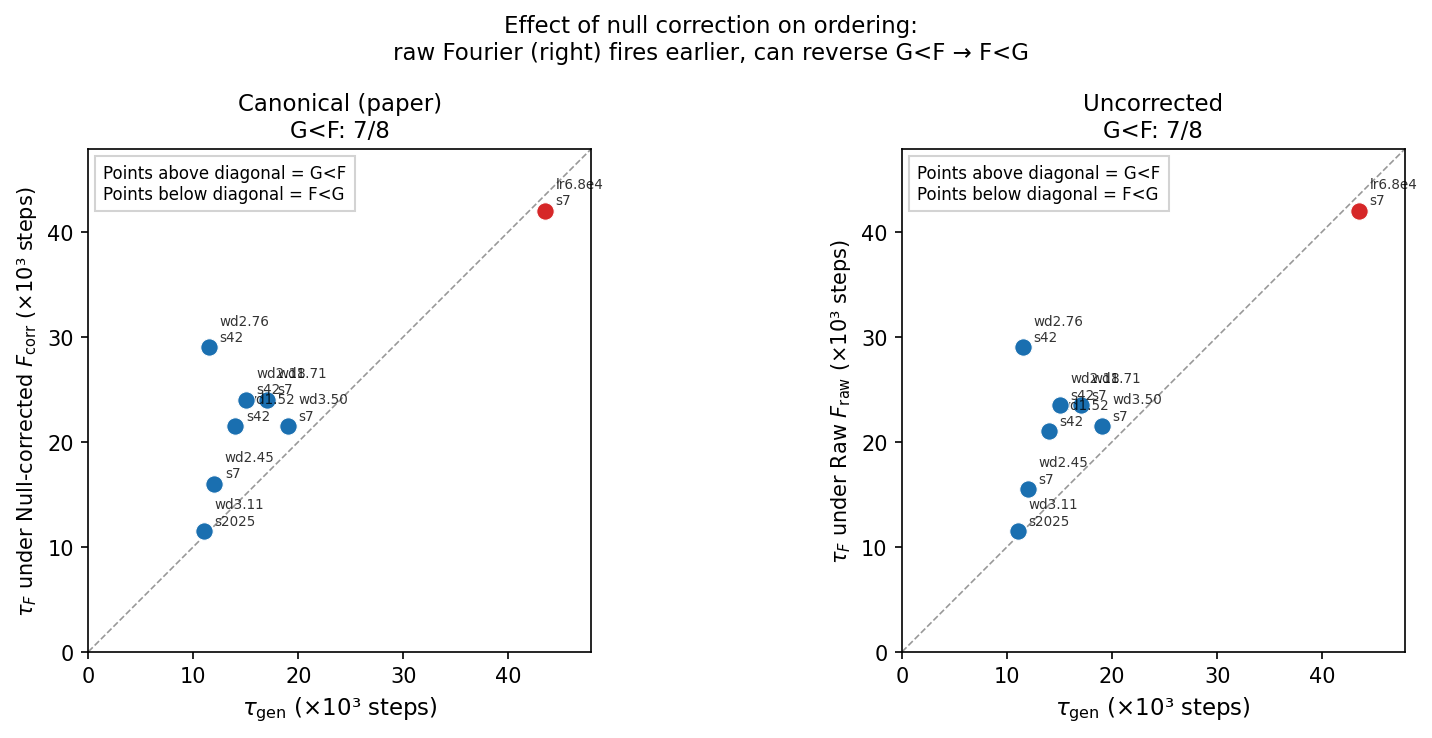
\includegraphics[width=0.85\textwidth]{raw_vs_corr_scatter.png}
\caption{Scatter of $\tau_F$ under null-corrected (left) vs.\ raw (right)
  Fourier for 8 sensitivity cells. Points above the diagonal indicate
  G$<$F ordering; points below indicate F$<$G.
  Blue points remain G$<$F under both metrics; the red point (F$<$G
  outlier) remains below the diagonal.
  No ordering flips across the two metrics.}
\label{fig:raw_vs_corr_scatter}
\end{figure}

\subsection{Detector Robustness}
\label{sec:robustness}

A natural concern is whether the G$<$F finding depends on the specific
choice of detector hyperparameters: the null-update interval, the EMA
smoothing coefficient, and the BIC slope threshold.
To address this, we trained 8 representative cells spanning strong,
medium, and weak G$<$F cases, one coincident case, and the sole
stable F$<$G case, and applied all $3\times4\times3=36$ detector
configurations post-hoc to the same saved trajectories.

We define the \textbf{Robustness Score} $\mathrm{RS} = N_{G<F} /
N_{\mathrm{total}}$ for each cell, where $N_{\mathrm{total}}=36$.
Results are shown in Figure~\ref{fig:robustness_heatmap}.
The five cells with $|\Dtau|\geq5{,}000$ steps achieve
$\mathrm{RS}=1.00$ (36/36 configurations yield G$<$F).
The two cells with $|\Dtau|\approx2{,}000$--$3{,}000$ steps achieve
RS$=0.83$ and RS$=0.75$, with the remaining configurations
classifying as \emph{coincident} rather than F$<$G.
Crucially, \textbf{no G$<$F cell is ever classified as F$<$G}
under any configuration.
The mean RS across all seven non-F$<$G cells is \textbf{0.94},
confirming that the G$<$F finding forms a robustness plateau
over the detector parameter space.

\begin{figure}[h]
\centering
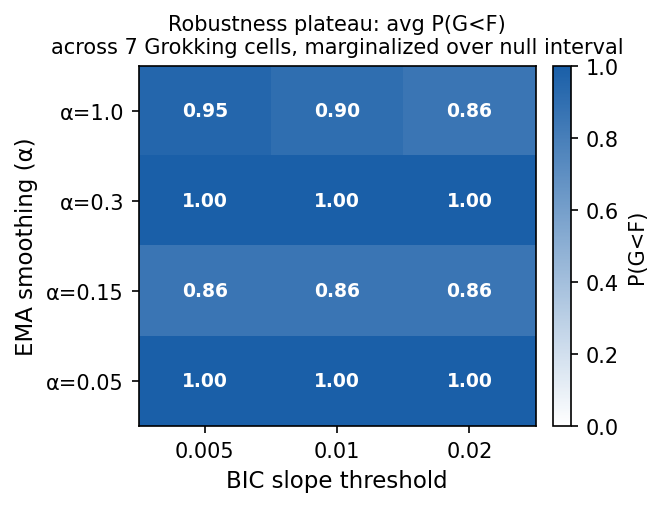
\includegraphics[width=0.52\textwidth]{sensitivity_robustness_heatmap.png}
\caption{%
  \textbf{Robustness plateau.}
  Each cell shows P(G$<$F) for a given (BIC slope threshold, EMA~$\alpha$)
  combination, averaged over null-update intervals \{500, 2500, 5000\}
  and over all seven Grokking cells.
  Strong and medium G$<$F cells achieve 1.00 across all configurations;
  weaker cells ($|\Dtau|\lesssim3{,}000$~steps) degrade gracefully to
  \emph{coincident}, never to F$<$G.
}
\label{fig:robustness_heatmap}
\end{figure}

\paragraph{The two F$<$G cases.}
Honest treatment requires acknowledging both F$<$G runs as genuine
in the metric sense, while characterizing what they reveal.

\textit{lr$=6.8\!\times\!10^{-4}$, seed~7} ($\Dtau=-1{,}500$,
RS$=0/36$).
All 36 detector configurations agree this is F$<$G, so the ordering
is stable and cannot be dismissed as a detection artifact.
However, trajectory inspection reveals that $\fcorr$ at $\taug$ is
only $0.015$---near the detection floor---while $\taug=43{,}500$
is the latest generalization time in our dataset.
At this very low learning rate, the weight-decay-to-learning-rate
ratio is $\mathrm{wd}/\mathrm{lr}\approx3{,}700$, compared to
$\approx1{,}070$ for a typical G$<$F cell.
A plausible interpretation is that strong relative weight decay
slowly compresses the embeddings toward Fourier-structured geometry
during the long wait before generalization, accumulating a barely
detectable $\fcorr$ signal before the sharp $\taug$ transition.
Whether this reflects a qualitatively different mechanism or an
extreme-parameter-ratio edge case of the same process requires
further investigation.

\textit{lr$=4.32\!\times\!10^{-3}$, seed~42} ($\Dtau=-54{,}500$,
RS not assessed).
This is the most extreme case: $\tauf=13{,}000$ but
$\taug=67{,}500$ (extended to 80k steps), with
max\_test\_acc$=0.965$ (below 1.0, indicating incomplete
generalization).
This run sits near the Grokking/Memorization phase boundary.
We conjecture that at high lr, the model can develop embedding
Fourier structure early---perhaps because weight decay acts more
aggressively on shallow features---while the slow, incomplete
generalization process unfolds on a much longer timescale.
This case may reflect genuinely different dynamics near the phase
boundary rather than the typical G$<$F consolidation regime, and
warrants a dedicated study.

Both cases occur near the boundaries of the Grokking phase
(low-lr edge and high-lr edge), suggesting the G$<$F ordering
is most reliable in the interior of the Grokking region
and may break down at the phase margins.

\subsection{Limitations}
\label{sec:limitations}

\paragraph{Single task.}
All experiments use $(a+b)\bmod 53$.
Generalization to other modular operations or non-modular tasks is open.

\paragraph{1D hyperparameter slices.}
Stages~2 and~3 cover one axis at a time.
A dense 2D grid would confirm G$<$F across the full Grokking region.

\paragraph{Measurement resolution.}
$\Dtau$ is measured with 500-step log-interval resolution;
small lags ($|\Dtau|\lesssim500$) cannot be reliably classified.
One F$<$G run has $|\Dtau|=1{,}500$ (three log-intervals),
which is above the resolution floor but small enough that caution
is warranted.

\paragraph{Circuit formation not measured.}
Our experiment measures only stages (2) and (3) of the proposed
three-stage picture.
We do not compute $\tau_{\text{circuit}}$ (the onset of the Fourier
computation mechanism in the attention and MLP layers), so the
claim that stage (1) precedes $\taug$ is borrowed from
\citet{nanda2023progress} rather than confirmed here.
Directly measuring all three timescales in the same runs---using
restricted logit loss or Fourier progress measures alongside our
embedding metric---is an important open direction.

\paragraph{Phase-boundary regime.}
Both F$<$G runs occur at the low-lr and high-lr margins of the
Grokking phase.
G$<$F may be specific to the interior of the Grokking region;
the ordering could be different near phase boundaries.
A denser sweep across both axes would clarify the boundary behavior.

% ==============================================================
\section{Conclusion}
\label{sec:conclusion}

We have shown that the token embedding Fourier geometry in grokked
transformers reliably consolidates \emph{after} generalization onset,
with G$<$F ordering in 52 of 55 Grokking runs (94.5\%) and a median
lag of $\approx7{,}000$ training steps.
This holds across two axes of the hyperparameter phase diagram,
suggesting it is a robust property of grokking in this setting rather
than an artifact of a specific hyperparameter choice.

Combined with the mechanism-level findings of \citet{nanda2023progress}
---who showed that the Fourier circuit forms before generalization---our
results paint a three-stage picture of grokking: mechanism formation,
generalization onset, then embedding-geometry consolidation.
The familiar Fourier ring in grokking visualizations reflects the
\emph{third} stage, not the \emph{first}.

A methodological takeaway: raw Fourier alignment triggers earlier and
can yield the opposite (F$<$G) ordering.
Null correction is essential for timing analyses of representation
structure.

\paragraph{Broader impact.}
This work studies a small-scale neural network training phenomenon.
No immediate harmful applications are foreseen.
Findings may inform training efficiency research by clarifying which
structural changes are or are not necessary for generalization.

% ==============================================================
\bibliography{refs}
\bibliographystyle{plainnat}

% ==============================================================
\appendix
\section{Experimental Details}
\label{app:details}

\subsection{BIC Changepoint Estimator}

We apply an exponential moving average ($\alpha{=}0.15$) to the
$\fcorr$ trajectory, then operate on $\log(1+t)$.
We search all candidate breakpoints in the interior two-thirds of
the sequence, fitting OLS regressions before and after each candidate.
The 4-parameter breakpoint model is accepted if BIC$_{\text{break}}
<$~BIC$_{\text{no-break}}$, where BIC$_k = n\log(\text{RSS}/n)
+ k\log(n)$.
A persistence check requires the post-break slope to exceed 1\% of
the total value range.

\subsection{Null Permutation Estimation}

Each run maintains a fixed NumPy RNG seeded as
$\text{run\_seed}\oplus\texttt{0xDEAD}$, independent of the model
RNG.
We shuffle the $p$ token indices 100 times every 5{,}000 steps to
estimate $F_{\mathrm{null,p95}}$.

\subsection{Hyperparameter Values}

\paragraph{Stage~2.}
wd~$\in\{1.20, 1.35, 1.52, 1.71, 1.93, 2.18, 2.45, 2.76, 3.11,
3.50\}$; lr~$=1.6\times10^{-3}$; seeds~$=\{42,7,2025\}$.

\paragraph{Stage~3.}
lr~$\in\{5.00, 6.80, 9.26, 12.6, 17.1, 23.3, 31.7, 43.2, 58.8,
80.0\}\times10^{-4}$; wd~$=2.5$; seeds~$=\{42,7,2025\}$.

% ==============================================================
\section{Complete Timing Results}
\label{app:scatter}

Figure~\ref{fig:tau_scatter} shows the full scatter of $(\taug,\tauf)$
for all 55~Grokking runs.
Points above the diagonal ($\tauf>\taug$) correspond to G$<$F;
the two red star ($\bigstar$) points below are the F$<$G cases discussed in
Section~\ref{sec:results_lr}.
The scatter confirms that the lag $\Dtau=\tauf-\taug$ is
distributed throughout the range 1{,}000--25{,}000 steps with no
obvious bimodal structure.

\begin{figure}[h]
  \centering
  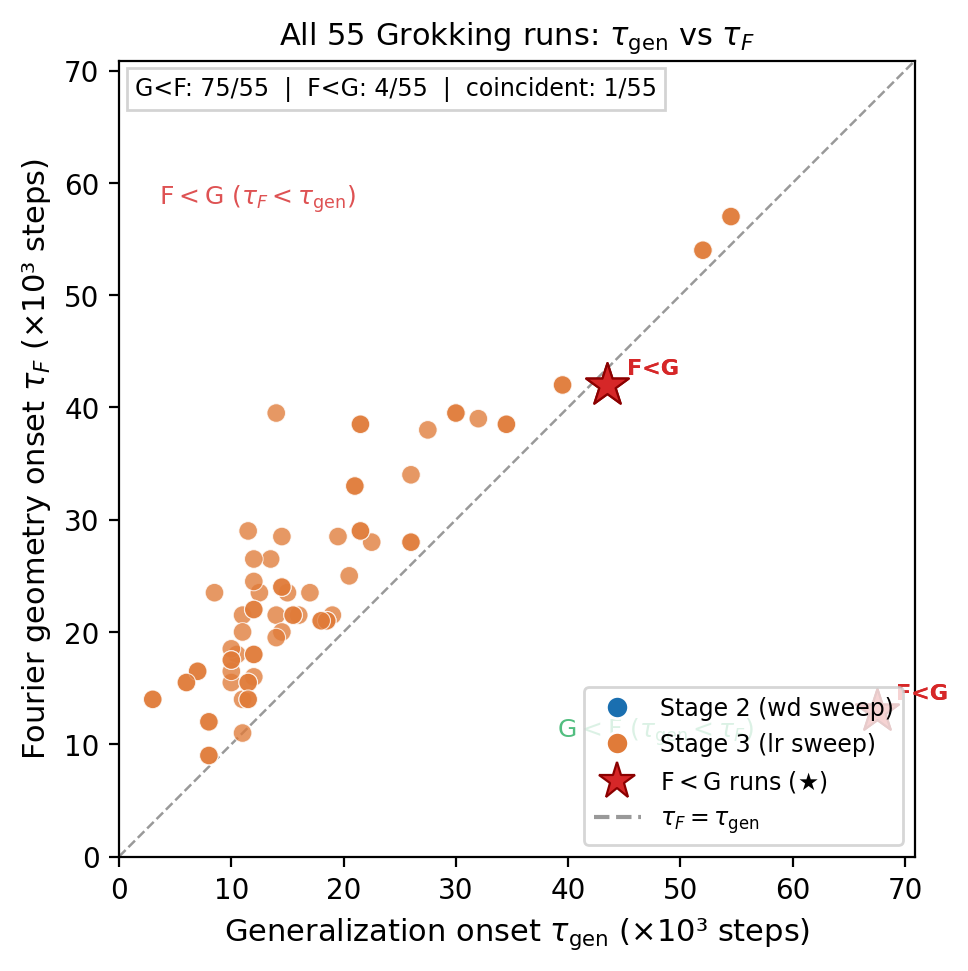
\includegraphics[width=0.58\linewidth]{tau_scatter.png}
  \caption{%
    Scatter plot of $\taug$ vs $\tauf$ for all 55~Grokking runs
    (blue = Stage~2 wd sweep; orange = Stage~3 lr sweep).
    All points above the dashed diagonal are G$<$F.
    The two red star ($\bigstar$) points below the diagonal are the
    F$<$G outliers discussed in Section~\ref{sec:results_lr}.
  }
  \label{fig:tau_scatter}
\end{figure}

% ==============================================================
\section{Per-Cell Detector Sensitivity}
\label{app:sensitivity}

Figure~\ref{fig:percell_heatmap} extends the aggregate
robustness heatmap (Figure~\ref{fig:robustness_heatmap}) to show
P(G$<$F) per cell, allowing inspection of which configurations
drive the RS~$<1$ cases.

\begin{figure}[h]
  \centering
  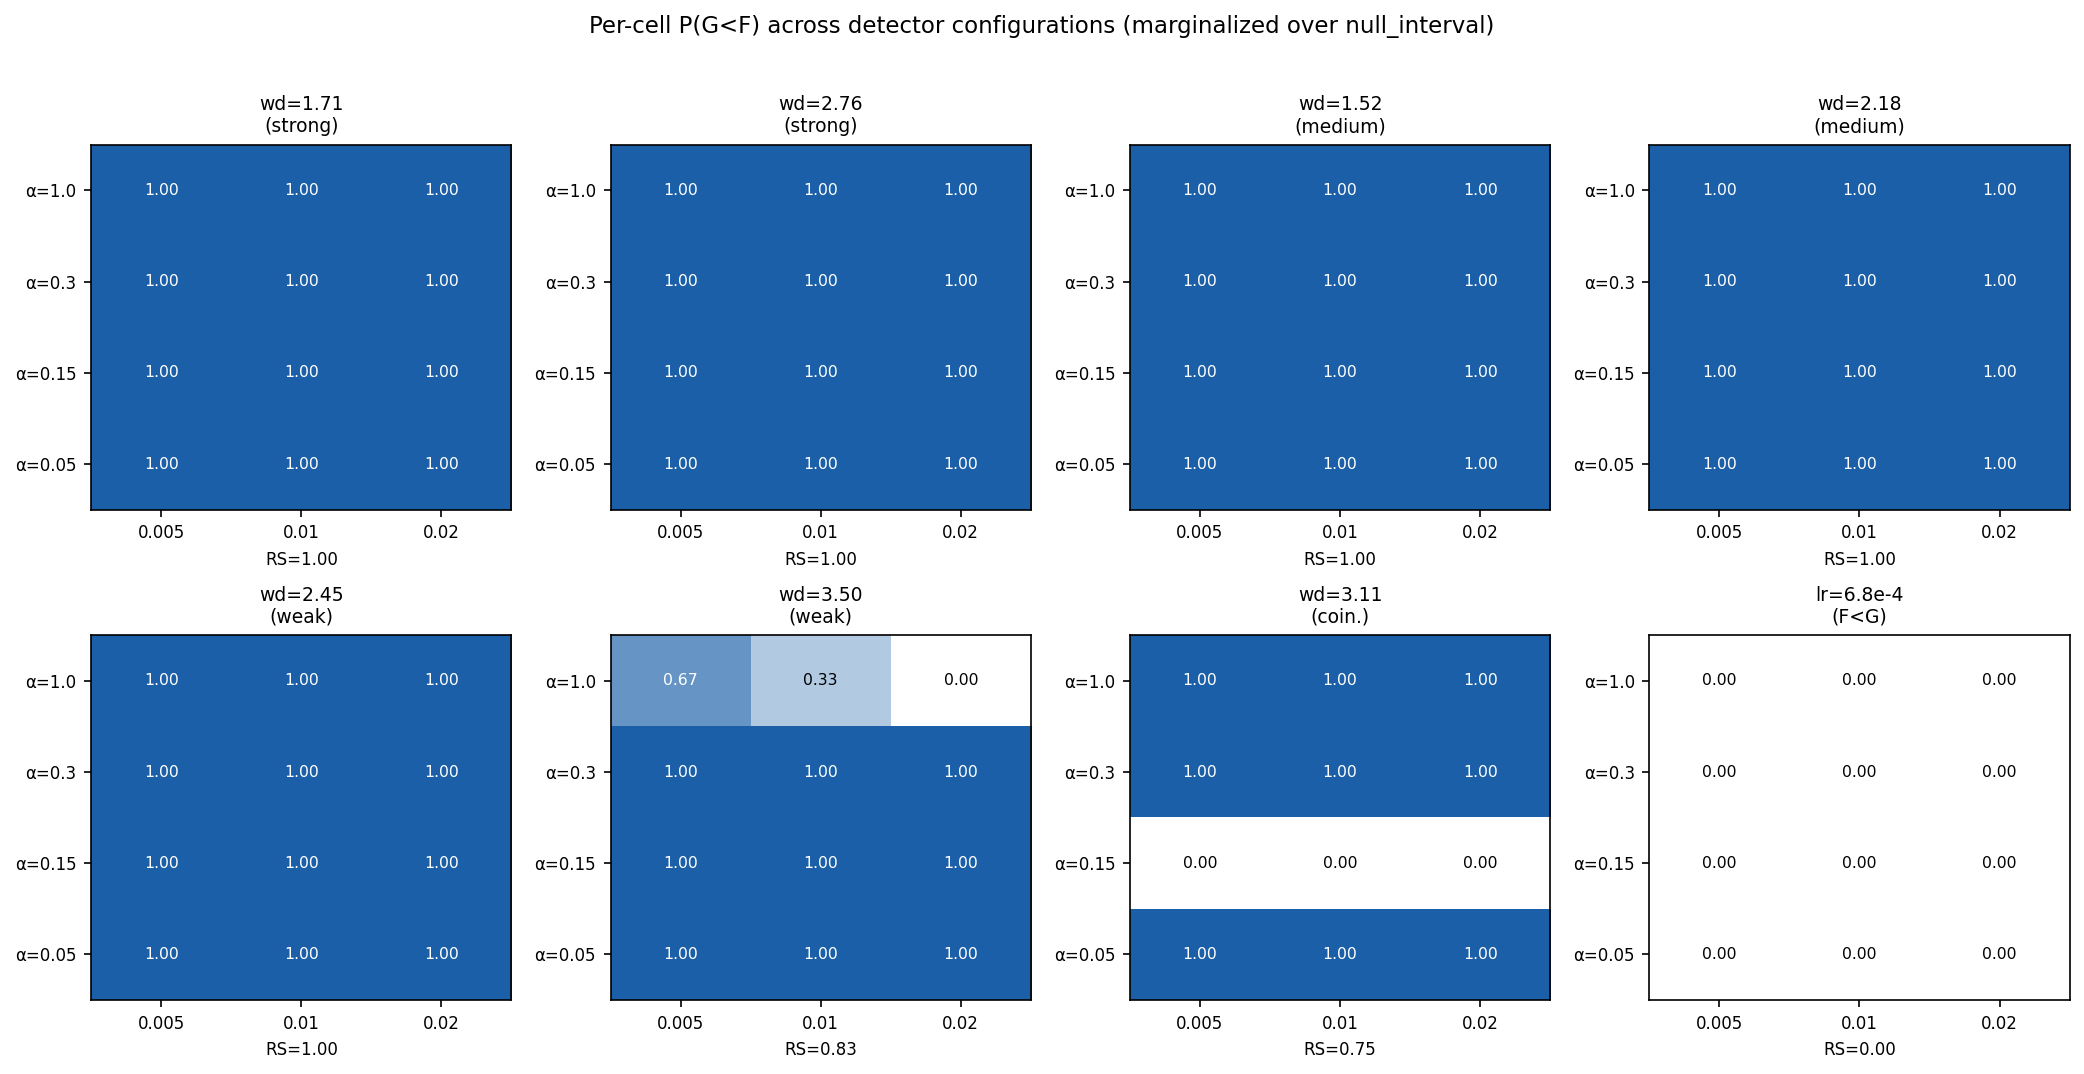
\includegraphics[width=\linewidth]{sensitivity_percell_heatmap.png}
  \caption{%
    Per-cell P(G$<$F) across all 36 detector configurations,
    marginalized over null-update interval.
    Strong and medium G$<$F cells (first four panels) are
    uniformly blue (RS$=1.00$).
    Weak G$<$F cells degrade to \emph{coincident} (not F$<$G)
    under the strictest slope threshold.
    The F$<$G outlier (bottom right) is uniformly red across
    all 36 configurations, confirming that its ordering is stable
    with respect to detector parameters.
  }
  \label{fig:percell_heatmap}
\end{figure}

Figure~\ref{fig:outlier_traj} provides a direct comparison of the
F$<$G outlier trajectory against the strong G$<$F reference cell.

\begin{figure}[h]
  \centering
  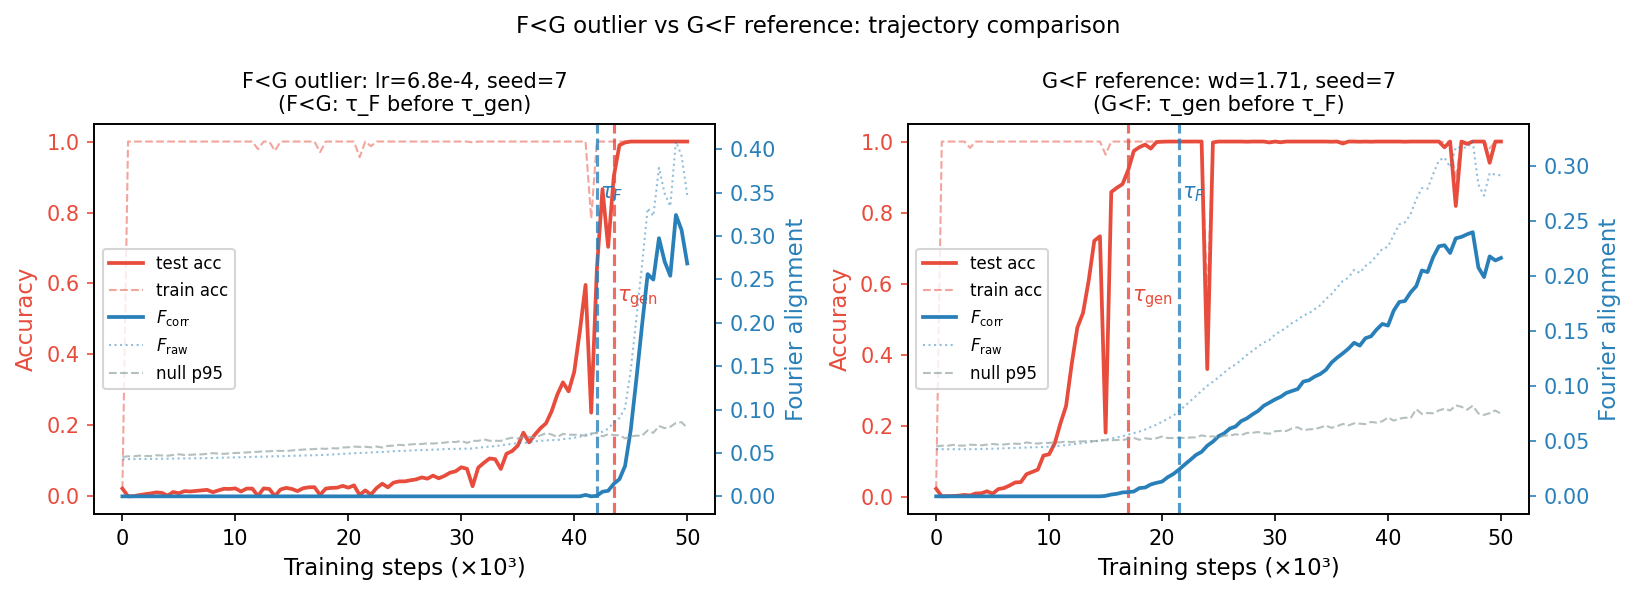
\includegraphics[width=0.90\linewidth]{sensitivity_outlier_trajectory.png}
  \caption{%
    Trajectory comparison: F$<$G outlier (lr$=6.8\!\times\!10^{-4}$,
    seed~7; left) vs.\ a strong G$<$F reference
    (wd$=1.71$, seed~7; right).
    In the outlier, $F_{\mathrm{raw}}$ (dotted blue) hovers near the
    null baseline (grey dashed) throughout training and $\fcorr$ only
    barely exceeds zero near the very late $\taug=43{,}500$.
    In the reference cell, $\fcorr$ shows a clear, sustained rise
    well after the sharp test-accuracy jump.
  }
  \label{fig:outlier_traj}
\end{figure}

\end{document}
